\documentclass[conference]{IEEEtran}

\usepackage{cite}
\usepackage{amsmath,amssymb}
\usepackage{graphicx}
\usepackage{booktabs}
\usepackage{url}
\usepackage{tikz}
\usetikzlibrary{arrows.meta}

\begin{document}

\title{Qwen2.5-72B: Architecture, Training, and\\Efficiency of an Open Dense Language Model}

\author{\IEEEauthorblockN{Nagham Taweel}
\IEEEauthorblockA{NLP \& AI Internship, Cellula Technologies\\
naghamatawel@gmail.com}}

\maketitle

\begin{abstract}
Qwen2.5-72B is the largest open-weight dense model of the Qwen2.5 family released by the Qwen Team at Alibaba. This paper analyzes its architecture, training methodology, and efficiency using the official technical report and model documentation. The model is an 80-layer decoder-only Transformer with 72.7B parameters that combines grouped query attention (GQA) with 64 query and 8 key-value heads, rotary position embeddings, SwiGLU feed-forward networks, RMSNorm pre-normalization, and QKV bias. It was pre-trained on 18 trillion tokens, more than twice the 7 trillion of Qwen2, and post-trained with over one million supervised examples followed by offline and online reinforcement learning. Dual Chunk Attention and YaRN extend its context from 32K to 128K tokens without further training. We derive its parameter count, key-value cache size, and compute cost from the published configuration, and we compare it with Qwen2-72B and Llama-3.1-405B. The instruction-tuned model matches or exceeds the five-times-larger Llama-3.1-405B on several benchmarks, showing that data quality and post-training can substitute for scale.
\end{abstract}

\begin{IEEEkeywords}
Qwen2.5, large language models, Transformer, grouped query attention, long context, reinforcement learning
\end{IEEEkeywords}

\section{Introduction}
Qwen2.5 is a series of large language models (LLMs) developed by the Qwen Team at Alibaba~\cite{qwen25}. It includes open-weight dense models in seven sizes (0.5B, 1.5B, 3B, 7B, 14B, 32B, and 72B), each released as a base and an instruction-tuned model, together with quantized versions; over 100 models are available on Hugging Face, ModelScope, and Kaggle~\cite{qwen25}. Two proprietary mixture-of-experts variants, Qwen2.5-Turbo and Qwen2.5-Plus, are served through Alibaba Cloud~\cite{qwen25}. The flagship open model, Qwen2.5-72B, is released under the Qwen license~\cite{qwen25,qwen25card}.

Compared with Qwen2~\cite{qwen2}, Qwen2.5 keeps the same dense architecture but improves almost everything around it: the pre-training data grows from 7T to 18T tokens, post-training adds a two-stage reinforcement learning (RL) pipeline, and generation length increases to 8K tokens~\cite{qwen25}. The model targets general chat, mathematics, coding, long-text generation, structured data such as tables and JSON, and multilingual use~\cite{qwen25}. This paper explains how its components work and interact, and why a 72B model can compete with much larger ones.

\section{Model Architecture}
Qwen2.5-72B is a decoder-only Transformer. Each of its 80 layers applies attention and a feed-forward network (FFN), each wrapped in RMSNorm pre-normalization and a residual connection (Fig.~\ref{fig:arch})~\cite{qwen25}:
\begin{align}
\mathbf{h}&=\mathbf{x}+\mathrm{Attn}\!\left(\mathrm{RMSNorm}(\mathbf{x})\right),\\
\mathbf{y}&=\mathbf{h}+\mathrm{FFN}\!\left(\mathrm{RMSNorm}(\mathbf{h})\right),
\end{align}
where RMSNorm rescales a vector by its root mean square, $\mathrm{RMSNorm}(\mathbf{x})=\mathbf{g}\odot\mathbf{x}/\sqrt{\tfrac{1}{d}\sum_i x_i^2+\epsilon}$, with a learned gain $\mathbf{g}$~\cite{rmsnorm}. Unlike LayerNorm, it does not subtract the mean, which makes it cheaper, and applying it before each sub-layer keeps training stable~\cite{qwen25}.

\textbf{Specifications.} The model has a hidden size of 8192, an FFN size of 29{,}568, 64 query heads and 8 key-value heads of dimension 128, and untied input and output embeddings~\cite{qwen2,qwen25card}. Table~\ref{tab:spec} compares it with Llama-3.1-405B. Qwen2-72B uses the same dimensions~\cite{qwen2}, so the improvements of Qwen2.5 come from data and training rather than from architectural changes.

\textbf{Parameter count.} The published values can be checked from the configuration. Each SwiGLU FFN has three $8192\times29{,}568$ matrices (about 727M parameters). Each attention layer has query and output projections of $8192\times8192$ and key and value projections of $8192\times1024$ (about 151M parameters). Over 80 layers this gives about 70.2B parameters, which matches the 70.0B non-embedding parameters reported in~\cite{qwen25card}. The two untied embedding matrices of $152{,}064\times8192$ add about 2.5B, giving the total of 72.7B.

\begin{figure}[t]
\centering
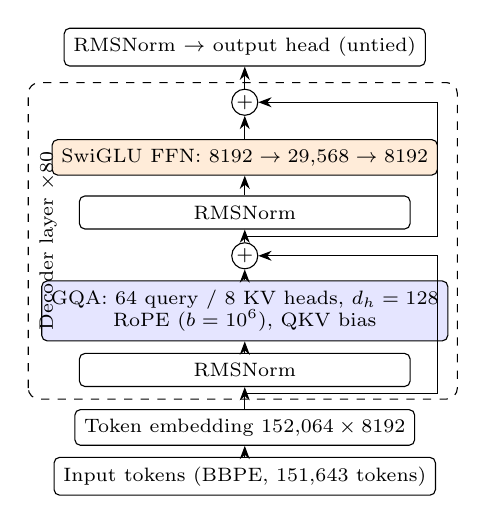
\begin{tikzpicture}[font=\scriptsize, >=Stealth,
  blk/.style={draw, rounded corners=2pt, minimum width=4.2cm, minimum height=0.42cm, align=center}]
\node[blk] (in) at (0,0) {Input tokens (BBPE, 151{,}643 tokens)};
\node[blk] (emb) at (0,0.62) {Token embedding $152{,}064\times8192$};
\node[blk] (n1) at (0,1.35) {RMSNorm};
\node[blk, fill=blue!10] (att) at (0,2.1) {GQA: 64 query / 8 KV heads, $d_h=128$\\RoPE ($b=10^6$), QKV bias};
\node[draw, circle, inner sep=0.5pt] (p1) at (0,2.8) {$+$};
\node[blk] (n2) at (0,3.35) {RMSNorm};
\node[blk, fill=orange!15] (ffn) at (0,4.05) {SwiGLU FFN: $8192\rightarrow29{,}568\rightarrow8192$};
\node[draw, circle, inner sep=0.5pt] (p2) at (0,4.75) {$+$};
\node[blk] (out) at (0,5.45) {RMSNorm $\rightarrow$ output head (untied)};
\draw[->] (in) -- (emb);
\draw[->] (emb) -- (n1);
\draw[->] (n1) -- (att);
\draw[->] (att) -- (p1);
\draw[->] (p1) -- (n2);
\draw[->] (n2) -- (ffn);
\draw[->] (ffn) -- (p2);
\draw[->] (p2) -- (out);
\draw[->] (0,1.05) -- (2.45,1.05) -- (2.45,2.8) -- (p1.east);
\draw[->] (0,3.05) -- (2.45,3.05) -- (2.45,4.75) -- (p2.east);
\draw[dashed, rounded corners] (-2.75,0.98) rectangle (2.7,5.0);
\node[rotate=90] at (-2.5,2.99) {Decoder layer $\times80$};
\end{tikzpicture}
\caption{Qwen2.5-72B decoder layer, based on~\cite{qwen25,qwen2,qwen25card}. Attention and the FFN each use RMSNorm pre-normalization and a residual connection.}
\label{fig:arch}
\end{figure}

\section{Attention Mechanism}
\textbf{Grouped query attention.} In standard multi-head attention (MHA), every query head has its own key and value heads, and all of them must be cached during generation. GQA lets a group of query heads share one key-value head~\cite{gqa}. Qwen2.5-72B uses $n_q=64$ query heads and $n_{kv}=8$ key-value heads, so each group of eight query heads shares one key-value pair~\cite{qwen25card}. For query head $i$ with group $g(i)=\lceil i/8\rceil$,
\begin{equation}
\mathrm{head}_i=\mathrm{softmax}\!\left(\frac{\mathbf{Q}_i\mathbf{K}_{g(i)}^{\top}}{\sqrt{d_h}}\right)\mathbf{V}_{g(i)},\quad \mathbf{Q}_i=\mathbf{X}W^{Q}_i+\mathbf{b}^{Q}_i,
\end{equation}
where the bias terms $\mathbf{b}$ on the query, key, and value projections (QKV bias) are a distinctive Qwen choice~\cite{qwen25}. The key-value cache per token is
\begin{equation}
M_{KV}=2\cdot n_{kv}\cdot d_h\cdot L\cdot p,
\end{equation}
with $L=80$ layers and $p$ bytes per value. With BF16 ($p=2$), this is about 328\,KB per token, eight times less than the 2.6\,MB that MHA with 64 key-value heads would need. A full 128K-token context therefore needs about 43\,GB of cache instead of about 344\,GB. This is the main reason the Qwen2 report gives for adopting GQA: higher inference throughput~\cite{qwen2}.

\textbf{Rotary position embedding.} Positions are encoded with RoPE~\cite{rope}, which rotates each pair of query and key dimensions by an angle proportional to the token position $m$, using frequencies
\begin{equation}
\theta_j=b^{-2j/d_h},\qquad j=0,\dots,d_h/2-1.
\end{equation}
The dot product $\mathbf{q}_m^{\top}\mathbf{k}_n$ then depends only on the relative distance $m-n$. Qwen2.5 raises the base $b$ from 10{,}000 to 1{,}000{,}000 (adjusted base frequency, ABF), so the rotations stay distinguishable over long distances~\cite{qwen25}.

\textbf{Long context.} Pre-training uses 4,096-token sequences and then extends them to 32,768 tokens~\cite{qwen25}. Two training-free methods extend the window four times further, to 131,072 tokens. YaRN rescales the rotary frequencies and attention~\cite{yarn}, and Dual Chunk Attention (DCA) splits long sequences into chunks so that relative positions stay within the range seen in training~\cite{dca,qwen2}. Within 32K tokens, DCA produces the same result as normal attention~\cite{qwen2}. On RULER at 128K tokens, these methods raise Qwen2.5-72B-Instruct from 67.0 to 88.4~\cite{qwen25}. The model card enables YaRN with a scaling factor of 4 and notes that static YaRN may slightly hurt short texts~\cite{qwen25card}.

\section{Feed-Forward Network and Tokenization}
Each FFN uses SwiGLU~\cite{glu}, a gated linear unit with the SiLU activation:
\begin{equation}
\mathrm{FFN}(\mathbf{x})=W_2\left(\mathrm{SiLU}(W_1\mathbf{x})\odot W_3\mathbf{x}\right),
\end{equation}
where $\mathrm{SiLU}(z)=z\,\sigma(z)$ and $\odot$ is element-wise multiplication. The gate branch $W_1\mathbf{x}$ decides how much of the value branch $W_3\mathbf{x}$ passes through, which works better than a plain ReLU FFN~\cite{glu}. With an intermediate size of 29{,}568 (about $3.6\times$ the hidden size), the FFNs hold about 83\% of the non-embedding parameters.

The tokenizer is byte-level byte-pair encoding (BBPE) with 151,643 regular tokens. Because it works on bytes, any text can be encoded without unknown tokens. Qwen2.5 expands the control tokens from 3 to 22, adding two for tool use~\cite{qwen25}.

\section{Training Methodology}
\textbf{Pre-training data.} The corpus grows to 18T tokens. Qwen2-Instruct models filter data quality, data from Qwen2.5-Math and Qwen2.5-Coder improve mathematics and coding, and Qwen2-72B-Instruct generates filtered synthetic data~\cite{qwen25}. Over-represented domains such as e-commerce and social media are down-sampled, while technology, science, and academic text are up-sampled~\cite{qwen25}.

\textbf{Optimization.} Instead of tuning the learning rate and batch size by trial and error, the team fitted scaling laws that predict their best values from model size and data size, using dense models from 44M to 14B parameters trained on 0.8B to 600B tokens~\cite{qwen25}.

\textbf{Post-training.} Supervised fine-tuning uses over one million examples for two epochs at a sequence length of 32,768, with the learning rate decayed from $7\times10^{-6}$ to $7\times10^{-7}$~\cite{qwen25}. Offline RL then applies direct preference optimization (DPO) to about 150,000 preference pairs~\cite{qwen25}. DPO trains the policy $\pi_\theta$ directly on preferred and rejected answers $(y_w,y_l)$ without a separate reward model~\cite{dpo}:
\begin{equation}
\mathcal{L}_{\mathrm{DPO}}=-\log\sigma\!\left(\beta\log\frac{\pi_\theta(y_w|x)}{\pi_{\mathrm{ref}}(y_w|x)}-\beta\log\frac{\pi_\theta(y_l|x)}{\pi_{\mathrm{ref}}(y_l|x)}\right).
\end{equation}
Online RL uses group relative policy optimization (GRPO)~\cite{grpo}. Eight responses are sampled per query~\cite{qwen25}, and each response is scored against its group, $A_i=(r_i-\mathrm{mean}(\mathbf{r}))/\mathrm{std}(\mathbf{r})$, so no value network is needed~\cite{grpo}. The reward model scores truthfulness, helpfulness, conciseness, relevance, harmlessness, and debiasing~\cite{qwen25}.

\section{Inference and Performance}
\textbf{Compute and memory.} As a dense model, Qwen2.5-72B uses all of its parameters for every token, about $2\times70$B $\approx140$ GFLOPs per forward pass by the common $2N$ estimate. Attention adds a cost that grows with context length. The BF16 weights need about 145\,GB, so serving needs several GPUs, while the released quantized versions reduce this cost~\cite{qwen25}. GQA keeps the cache small (Section~III), and vLLM is the recommended serving engine~\cite{qwen25card}. For the proprietary Qwen2.5-Turbo, a sparse attention method reduces attention computation by $12.5\times$ for 1M-token inputs~\cite{qwen25}.

\textbf{Benchmarks.} Table~\ref{tab:bench} shows that Qwen2.5-72B-Instruct improves strongly over Qwen2-72B-Instruct, with MATH rising from 69.0 to 83.1 and Arena-Hard from 48.1 to 81.2. It also beats Llama-3.1-405B-Instruct on MMLU-redux, MATH, MBPP, LiveCodeBench, and Arena-Hard~\cite{qwen25}. The larger model still leads on MMLU-Pro, GPQA, and IFEval. As a base model, Qwen2.5-72B reaches 86.1 on MMLU compared with 85.2 for Llama-3-405B~\cite{qwen25}.

\begin{table}[t]
\centering
\caption{Architecture of Qwen2.5-72B and Llama-3.1-405B~\cite{qwen25,qwen2,qwen25card,llama3}}
\label{tab:spec}
\begin{tabular}{lcc}
\toprule
 & Qwen2.5-72B & Llama-3.1-405B \\
\midrule
Parameters & 72.7B & 405B \\
Layers & 80 & 126 \\
Hidden / FFN size & 8192 / 29{,}568 & 16{,}384 / 53{,}248 \\
Query / KV heads & 64 / 8 & 128 / 8 \\
Vocabulary & 151{,}643 + 22 & 128K \\
Context length & 128K & 128K \\
Pre-training tokens & 18T & 15.6T \\
\bottomrule
\end{tabular}
\end{table}

\begin{table}[t]
\centering
\caption{Instruction-tuned models, from~\cite[Table~6]{qwen25}}
\label{tab:bench}
\setlength{\tabcolsep}{5pt}
\begin{tabular}{lcccc}
\toprule
Benchmark & Qwen2.5 & Qwen2 & Llama-3.1 & Llama-3.1 \\
 & 72B & 72B & 70B & 405B \\
\midrule
MMLU-Pro & 71.1 & 64.4 & 66.4 & \textbf{73.3} \\
MMLU-redux & \textbf{86.8} & 81.6 & 83.0 & 86.2 \\
GPQA & 49.0 & 42.4 & 46.7 & \textbf{51.1} \\
MATH & \textbf{83.1} & 69.0 & 68.0 & 73.8 \\
HumanEval & 86.6 & 86.0 & 80.5 & \textbf{89.0} \\
MBPP & \textbf{88.2} & 80.2 & 84.2 & 84.5 \\
LiveCodeBench & \textbf{55.5} & 32.2 & 32.1 & 41.6 \\
IFEval & 84.1 & 77.6 & 83.6 & \textbf{86.0} \\
Arena-Hard & \textbf{81.2} & 48.1 & 55.7 & 69.3 \\
\bottomrule
\end{tabular}
\end{table}

\section{Key Innovations}
Qwen2.5-72B uses components that are now standard, but it differs from other LLMs in four ways:
\begin{enumerate}
\item \emph{Data over scale:} 18T carefully filtered tokens, with model-based quality filtering and domain rebalancing, allow a 72B model to compete with the 405B Llama 3.1, which was trained on 15.6T tokens~\cite{qwen25,llama3}.
\item \emph{Efficient attention:} GQA with an 8:1 ratio, QKV bias, and RoPE with a base of $10^6$, combined with training-free YaRN and DCA, give 128K context at a modest memory cost~\cite{qwen25,qwen2}.
\item \emph{Scaling-law hyper-parameters:} the learning rate and batch size are predicted rather than searched~\cite{qwen25}.
\item \emph{Two-stage RL:} offline DPO for reasoning skills, followed by online GRPO for helpfulness and safety~\cite{qwen25}.
\end{enumerate}

\section{Conclusion}
Qwen2.5-72B shows that a well-understood dense Transformer can reach frontier-level results through better data and training rather than more parameters. Its GQA attention, SwiGLU FFNs, and RMSNorm pre-normalization keep the design simple and efficient, while YaRN and DCA extend it to 128K tokens without retraining. Its main costs are the 145\,GB of BF16 weights and the dense compute per token, which the proprietary MoE variants Qwen2.5-Turbo and Qwen2.5-Plus are designed to reduce~\cite{qwen25}.

\bibliographystyle{IEEEtran}
\bibliography{references}

\end{document}
